\documentclass{article}%
\usepackage[T1]{fontenc}%
\usepackage[utf8]{inputenc}%
\usepackage{lmodern}%
\usepackage{textcomp}%
\usepackage{lastpage}%
\usepackage[head=40pt,margin=0.5in,bottom=0.6in]{geometry}%
\usepackage{graphicx}%
%
\title{\textbf{Ortega Díaz propone al Parlamento realizar enmienda constitucional}}%
\author{Rafael León}%
\date{07/10/2018}%
%
\begin{document}%
\normalsize%
\maketitle%
\textbf{URL: }%
http://www.el{-}nacional.com/noticias/politica/ortega{-}diaz{-}propone{-}parlamento{-}realizar{-}enmienda{-}constitucional\_254698\newline%
%
\textbf{Periodico: }%
EN, %
ID: %
254698, %
Seccion: %
Política\newline%
%
\textbf{Palabras Claves: }%
Política, Asamblea Nacional, Luisa Ortega Díaz\newline%
%
\textbf{Derecho: }%
CONTEXTO, %
Otros Derechos: %
, %
Sub Derechos: %
\newline%
%
\textbf{EP: }%
NO\newline%
\newline%
%
\textbf{\textit{La fiscal general indicó que se debe detener el proyecto constituyente que adelanta el gobierno y la ANC}}%
\newline%
\newline%
%
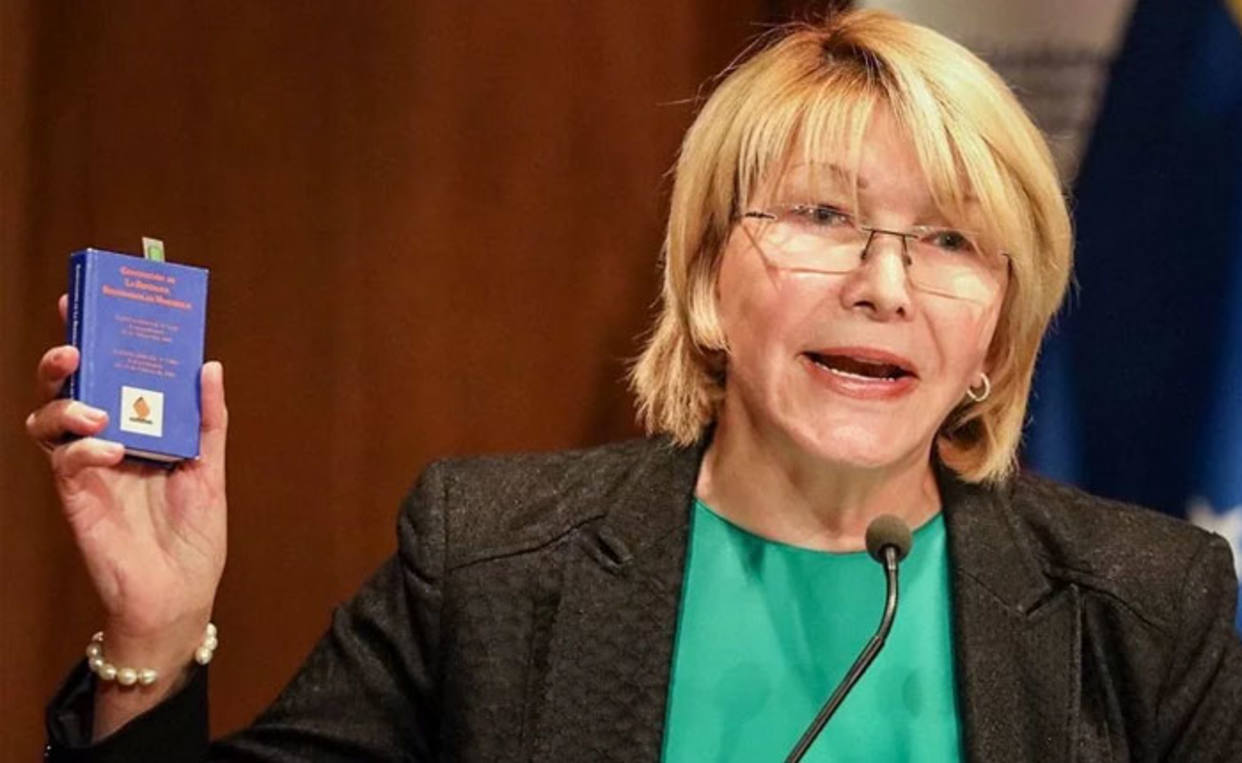
\includegraphics[width=300px]{17.jpg}%
\newline%
%
La fiscal general, destituida por la asamblea nacional constituyente, Luisa Ortega Díaz propuso a~la Asamblea Nacional~llevar a cabo una enmienda de~la Constitución~para impedir que el gobierno del presidente Nicolás Maduro derogue la carta magna vigente.%
\newline%
%
“He propuesto a los factores políticos y sociales que, en el marco de las facultades de la Asamblea Nacional, único poder legítimo que queda en el país, se convoque a una enmienda constitucional para impedir expresamente que se reforme, derogue, cambie o pierda vigencia la actual Constitución por un lapso de cinco años”, explicó a través de un video difundido en Twitter.%
\newline%
%
Ortega Díaz alertó que con el proyecto constituyente que adelanta el gobierno “se sellará la destrucción definitiva de Venezuela”. Advirtió que en los próximos seis meses se llamará a elecciones para aprobar una nueva Constitución y afirmó que, de ser así, los venezolanos perderán todos sus derechos y se consolidará el totalitarismo en el país.%
\newline%
%
Desde el exilio, la ex funcionaria pidió la unidad de todos los sectores de la sociedad a quienes llamó a “no quedarse de brazos cruzados” y defender~la Constitución~vigente.%
\newline%
%
\end{document}